\label{es314}
\begin{flushleft}
Nel primo caso abbiamo usato la matrice $A\in M^{3\times 3}$ con elementi:
\[ 
A =
\begin{pmatrix}
    0 & -3 &  8 \\
   -1  &  8  &  7 \\
    1  &  3  &  0 \\
\end{pmatrix}
\]
e il vettore dei termini noti $b\in \mathbb{R}^3$ con valori:
\[
b = \begin{pmatrix}
    3.1416 \\
    1.1618 \\
    2.7183 \\
\end{pmatrix}
\]
Nel secondo caso abbiamo usato la matrice $A\in M^{3\times 3}$ con elementi:
\[ 
A =
\begin{pmatrix}
    14 & 5 &  2 \\
    5 &  8  &  1 \\
    2  &  1  &  4 \\
\end{pmatrix}
\]
e il vettore dei termini noti $b\in \mathbb{R}^3$ con valori:
\[
b = \begin{pmatrix}
    3.1416 \\
    1.1618 \\
    2.7183 \\
\end{pmatrix}
\]
Usando il codice MatLab sottostante è possibile risolvere questi 2 esempi:
\lstinputlisting[language=Matlab]{cap_3/es14/es14.m}
Il codice sopra restituisce l'output:
\begin{figure}[H]
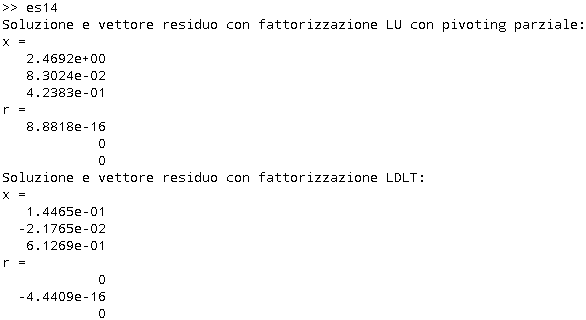
\includegraphics[left, width=300px]{cap_3/es14/es314.png}
\end{figure}
\end{flushleft}